\documentclass{article}
\usepackage{graphicx}
\usepackage{titling}
\usepackage[margin=1in]{geometry}
\usepackage{array}
\usepackage{fancyhdr}

\newcommand{\subtitle}[1]{%
  \posttitle{%
    \par\end{center}
    \begin{center}\large#1\end{center}
    \vskip0.5em}%
}

\pagestyle{fancy}
\fancyhf{}
\fancyfoot[C]{General Operations Over Basic Embedded Radio -- 1.00.0}
\fancyfoot[R]{\thepage}
\renewcommand{\headrulewidth}{0pt}
\renewcommand{\footrulewidth}{0.4pt}

\title{
  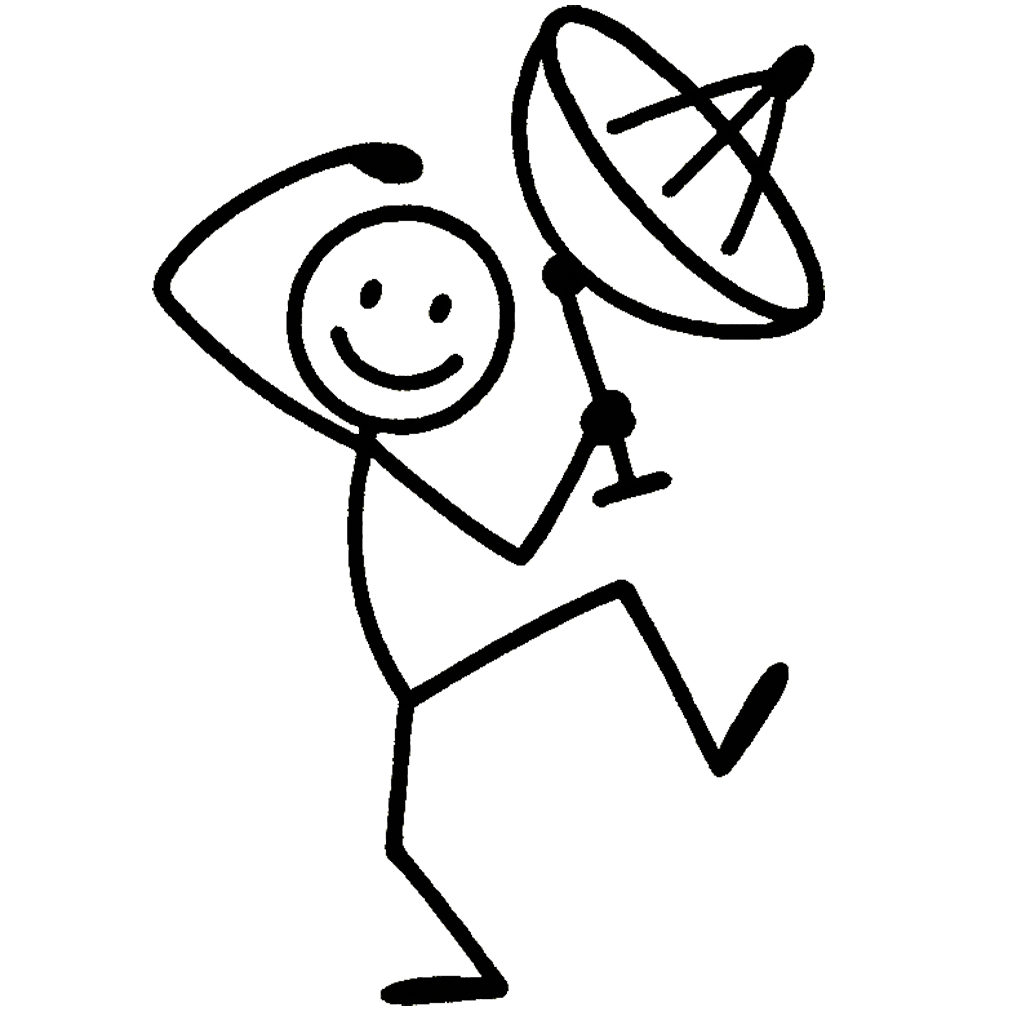
\includegraphics[width=0.25\linewidth]{goober logo.png}\\[0.5em]
  \textbf{General Operations Over Basic Embedded Radio}
}
\subtitle{A lightweight digital communications protocol.}
\author{Abdul Zia, Arizona State University}
\date{November 26th, 2025 \\ Version 1.00.0}

\begin{document}
\maketitle
\thispagestyle{fancy}

\newpage

\section{Introduction}

\noindent
The General Operations Over Basic Embedded Radio (abbreviated GOOBER) protocol is designed for use in vehicle avionics. The GOOBER protocol is a specification that dictates how command and control exchanges should take place between devices communicating on the same frequency, channel, or bus.
\\\\
GOOBER is designed to communicate through various physical layers such as LoRa, 4G LTE, TCP/UDP, Bluetooth, etc. to create a network of interconnected devices.
\\\\
While networking multiple devices is the end goal, GOOBER's purpose is to accommodate one-way, half-duplex, and full-duplex communications between devices on a shared communication path.
\\\\
GOOBER is not sophisticated by nature. It is created with simplicity and expandability in mind. It should be easy to implement into any embedded system.


\section{Packet Structure}

\noindent
At its core, GOOBER is just a structure of bytes arranged in a meaningful manner. The structure of a GOOBER packet is shown below.
\\

\begin{table}[h]
    \centering
    \begin{tabular}{|c|c|c|c|c|c|}
        \hline

        \textbf{Name} 
            & DEV\_ID & DEV\_MODE & SEQ\_ID & MSG\_CLS & PAYLOAD\\ \hline

        \textbf{Size (bytes)}
            & 1 & 1 & 1 & 1 & 1 + n \\ \hline

        \textbf{Offset (bytes)} 
            & 0 & 1 & 2 & 3 & 4 \\ \hline
    \end{tabular}
\end{table}

\noindent For a detailed description of each byte's structure and usage, see the below subsections.

\subsection{DEV\_ID}
Each device on the GOOBER network has a unique device ID, represented as an unsigned integer of 8 bits. This can be any number between 0 and 255, allowing a maximum of 256 devices in one network.
\\\\
The DEV\_ID byte uses the following arrangement:

\begin{table}[h]
    \centering
    \begin{tabular}{|c|c|c|c|c|c|c|c|c|}
    \hline
    \textbf{Bit}
        & 0 & 1 & 2 & 3 & 4 & 5 & 6 & 7 \\ \hline
    \textbf{Value}
    & ID[0] & ID[1] & ID[2] & ID[3] & ID[4] & ID[5] & ID[6] & ID[7]\\ \hline
    \end{tabular}
\end{table}

\noindent Device IDs are important in identifying where a GOOBER packet originates from, and should not be duplicated across devices on the same network. Unique device IDs are crucial for allowing receivers to relay information across multiple physical layers.
\\\\
It is recommended to segment device IDs based on the different physical layers present in a network. For example, devices 0-16 can be reserved for LoRa radios, devices 17-32 can be reserved for Bluetooth devices, and so on.
\\\\

\subsection{DEV\_MODE}
Transmissions on the GOOBER network can be one-way, half-duplex, or full duplex. The DEV\_MODE byte ensures that transmitters and receivers use proper sequencing to avoid conflicts when using a shared communication path.
\\\\
Device mode 0 is an invalid/error mode. Device mode 1 indicates a one-way link. Device mode 2 indicates a half-duplex link. Device mode 3 indicates a full-duplex link.
\\\\
The DEV\_MODE byte uses the following arrangement:

\begin{table}[h]d
    \centering
    \begin{tabular}{|c|c|c|c|c|c|c|c|c|}
    \hline
    \textbf{Bit}
        & 0 & 1 & 2 & 3 & 4 & 5 & 6 & 7 \\ \hline
    \textbf{Value}
        & Device Mode LSB & Device Mode MSB & Intent Bit & Rsvd. & Rsvd. & Rsvd. & Rsvd. & Rsvd.\\ \hline
    \end{tabular}
\end{table}

\begin{itemize}
    \item Bit 0: Device mode LSB.
    \item Bit 1: Device mode MSB.
    \item Bit 2: Intent bit. This is used in half-duplex communication. When this bit is 1, the transmitting device indicates that it intends to transmit another packet on the same communication path immediately.
    \item Bits 3-7: Reserved for future use.
\end{itemize}

\subsection{SEQ\_ID}
The SEQ\_ID byte is an unsigned 8-bit integer that increments with each transmission. This allows receivers to detect if any packets were dropped or received out of order during communication.
\\\\
The SEQ\_ID byte uses the following arrangement:

\begin{table}[h]
    \centering
    \begin{tabular}{|c|c|c|c|c|c|c|c|c|}
    \hline
    \textbf{Bit}
        & 0 & 1 & 2 & 3 & 4 & 5 & 6 & 7 \\ \hline
    \textbf{Value}
    & SEQ[0] & SEQ[1] & SEQ[2] & SEQ[3] & SEQ[4] & SEQ[5] & SEQ[6] & SEQ[7]\\ \hline
    \end{tabular}
\end{table}

\noindent The sequence ID wraps around from 255 to 0 after reaching its maximum value. Each device maintains its own sequence counter that increments with every packet transmitted.
\\\\
The SEQ\_ID should not used to determine the timestamp of a transmission. It is not time dependent.

\subsection{MSG\_CLS}
The MSG\_CLS byte is an unsigned 8-bit integer ranging from 0x01 to 0xFE that indicates the message class of the payload being sent. Message classes are stored in a lookup table on each device and are application-dependent.
\\\\
Special values:
\begin{itemize}
    \item 0x00: Reserved.
    \item 0xFF: Reserved.
\end{itemize}

The MSG\_CLS byte uses the following arrangement:

\begin{table}[h]
    \centering
    \begin{tabular}{|c|c|c|c|c|c|c|c|c|}
    \hline
    \textbf{Bit}
        & 0 & 1 & 2 & 3 & 4 & 5 & 6 & 7 \\ \hline
    \textbf{Value}
    & CLS[0] & CLS[1] & CLS[2] & CLS[3] & CLS[4] & CLS[5] & CLS[6] & CLS[7]\\ \hline
    \end{tabular}
\end{table}

\subsection{PAYLOAD}
The PAYLOAD section contains the actual data being transmitted. It consists of a length byte followed by the payload data.
\begin{itemize}
    \item \textbf{Length Byte}: The first byte is an unsigned 8-bit integer representing the length of the payload data in bytes (0-255).
    \item \textbf{Payload Data}: The remaining N bytes contain the actual message content, where N is the value specified in the length byte.
\end{itemize}

\noindent
The minimum payload size is 0 bytes. The maximum payload size is 250 bytes. This is to limit the overall size of a GOOBER packet to be less than 256 bytes.



\end{document}
